\section{基線長とその基線伸縮スペクトルの関係}
基線長伸縮は共振器の制御信号に乗るので、小さく低減されるのが望ましい。とくにRMSが大きい脈動は、制御を不安定にする主な原因となっており、それを低減するための工夫を必要とする。一つの簡単な方法は、共振器をブレッドボードに乗せることである。これにより2つの鏡同士は相関をもち、脈動のような低周波地面振動では同相で鏡が動くため、逆相成分が同相成分と比べて相対的に低減される。この考えに立つと、KAGRAの腕共振器も飛騨片麻岩の上に固定しており、ある程度相関をもっていると思われる。本章では、どの程度Xアームで逆相成分が低減されているか評価する。


\subsection{同相成分と逆相成分}
図\ref{img:img_diffcomm}で示すようなXアーム上の2点,$x_1,\,x_2$について,これら2つの同相成分$x_{\mathrm{com}}$と逆相成分$x_\mathrm{diff}$を
\begin{eqnarray}\label{eq:eq22}
  x_{\mathrm{diff}} &\equiv& \frac{x_{1}-x_{2}}{\sqrt{2}}, \\
  x_{\mathrm{com}}  &\equiv& \frac{x_{1}+x_{2}}{\sqrt{2}}
\end{eqnarray}
と定義する。パワーが保存するように、規格化定数は$\sqrt{2}$にしている。同相成分は,2点の重心移動をあらわし,逆相成分は2点の基線長伸縮を表す。


\begin{figure}[H]
  \begin{center}
    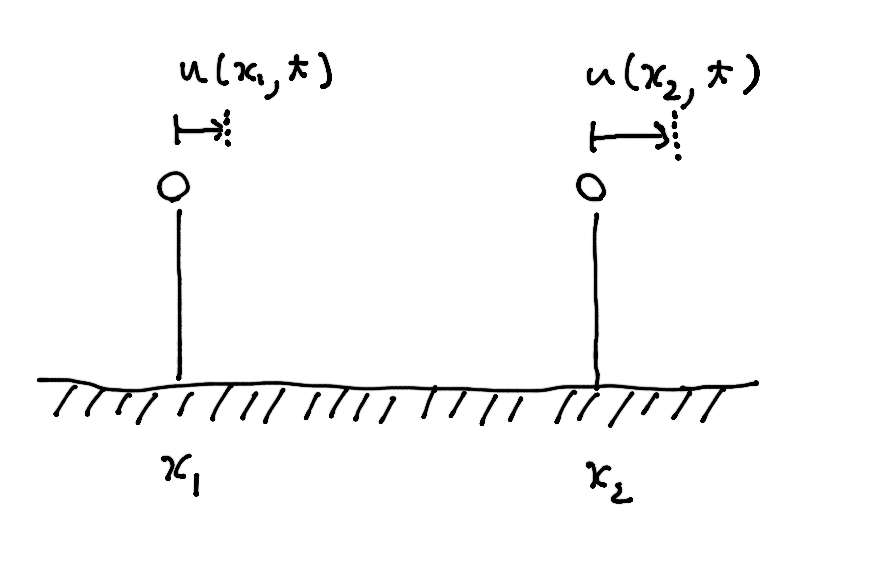
\includegraphics[width=11.5cm]{./XarmDifferentialSpectrum/xarm.png}
  \end{center}
  \caption{Xアーム上の2点の変位。それぞれの位置を$x_1,\,x_2$とすれば変位はそれぞれ$u(x_1,t),\,u(x_2,t)$となる。}\label{img:img_diffcomm}
\end{figure}


\subsection{Common Differential Mode Rate (CDMR)}
図\ref{img:img_diffcomm}上の2点$x_1,\,x_2$がコヒーレンスを持っている場合を考える。2点それぞれがノイズで埋もれている,つまり無相関な場合は,同相と逆相の成分比は1:1になる。一方でコヒーレンスが1の場合,2点の位相差は0度となり同相で動くので,逆相成分は消え,同相成分のみになる。コヒーレンスが−1の場合は,反対に逆相成分のみになる。このようにコヒーレンスは,同相と逆相の成分比と関係をもっている。


基線長伸縮がどの程度低減されているかを表す指標として,2つの信号の同相と逆相の振幅成分の比、Common Differential Mode Rate (CDMR) を
\begin{equation}
  \boxed{\mathrm{CDMR} \equiv \sqrt{\frac{同相成分のパワー}{逆相成分のパワー}} = \sqrt{\frac{P_{\mathrm{com}}(\omega)}{P_{\mathrm{diff}}(\omega)}}} \label{eq:eq23}
\end{equation}
と定義する。$P_{\mathrm{com}},P_{\mathrm{diff}}$は同相成分と逆相成分についてのパワースペクトル密度である。パワースペクトル密度は自己相関関数$C(\tau)$をフーリエ変換したものなので、まず自己相関関数$C_{\mathrm{diff}}$を求める。自己相関関数$C_{\mathrm{diff}}$は,各々の自己相関を$ C_{ij} \equiv \langle x_{i}(t)x_{j}(t+\tau)\rangle,\, (i=1,2,\,j=1,2)$と定義すれば, 
\begin{eqnarray}
  C_{\mathrm{diff}}(\tau) &=& \frac{1}{2}
  \langle
  \left[ x_{1}(t)-x_{2}(t) \right]   \left[ x_{1}(t+\tau)-x_{2}(t+\tau) \right]
  \rangle \\
  &=& \frac{1}{2}\left( C_{11}(\tau) - C_{12}(\tau) - C_{21}(\tau) + C_{22}(\tau) \right), 
\end{eqnarray}
となるので、これをフーリエ変換すれば逆相成分のパワースペクトル密度$P_{\mathrm{diff}}(\omega)$は
\begin{eqnarray}
  P_{\mathrm{diff}}(\omega) &=& \frac{1}{2}\left( P_{1}(\omega) + P_{2}(\omega) - X_{12}(\omega) - X_{12}^*(\omega) \right)\\
  &=& \frac{1}{2} \sqrt{P_{1}P_{2}} \left( \sqrt{\frac{P_{1}}{P_{2}}}+ \sqrt{\frac{P_{2}}{P_{1}}} - 2\Re \left[\mathrm{coh} \right] \right) , 
\mathrm{coh} \equiv \frac{X_{12}}{\sqrt{P_{1}P_{2}}} \label{eq:eq31}
\end{eqnarray}
となる。$P_{1}(\omega),P_{2}(\omega)$はパワースペクトル密度、$X_{12}(\omega)$はクロススペクトル密度、$\mathrm{coh}$はコヒーレンスである。


さて、2つの信号$x_{1},x_{2}$のパワーが同じ、つまり$P_{1}=P_{2}\equiv P$の場合、式(\ref{eq:eq31})はさらに計算できて、結果として$P_{\mathrm{diff}}$は
\begin{eqnarray}
 P_{\mathrm{diff}}(\omega) = P \left(1 - \Re \left[\mathrm{coh} \right] \right) \label{eq:eq35}
\end{eqnarray}
となる。同相成分も同様の計算をして、
\begin{eqnarray}
 P_{\mathrm{diff}}(\omega) = P \left(1 - \Re \left[\mathrm{coh} \right] \right) \label{eq:eq36}
\end{eqnarray}
となるので、$\mathrm{CDMR}$は定義式(\ref{eq:eq23})より、
\begin{eqnarray}
 \mathrm{CDMR} = \sqrt{\frac{1 + \Re \left[\mathrm{coh} \right] }{1 - \Re \left[\mathrm{coh} \right]}} \label{eq:eq33}
\end{eqnarray}
と書き表すことができる。
式(\ref{eq:eq33})が示すように、同相成分と逆相成分のパワー比は2つの信号のコヒーレンスであらわすことができる。


\subsubsection{平面波をノイズを含んで測定している場合}
CDMRはコヒーレンスで表すことができることがわかったので,次に具体的にコヒーレンスをもとめてみる。図\ref{img:img_diffcomm}中のXアームに沿った二点の上を,平面波が伝搬している場合を考える。


ノイズが同じ測定器でこの信号を測定すれば,変位はそれぞれ
\begin{eqnarray}
  x_1 = u(x_1,t) + n(t) \\
  x_2 = u(x_2,t) + n(t)
\end{eqnarray}
のように表すことができる。このときの$x_1$と$x_2$の相互相関関数$C_{12}$は,ノイズは信号と無相関になるので,
\begin{eqnarray}
  C_{12} = C_{u_1,u_2}
\end{eqnarray}
のように信号同士の相互相関関数で簡単に表すことできる。つまりコヒーレンスは
\begin{eqnarray}
  \mathrm{coh} \equiv \frac{X_{12}}{\sqrt{P_1P_2}} &=&
  \frac{X_{u_1,u_2}}{\sqrt{(P_{u1}+P_n)(P_{u2}+P_n)}} \\
  &=& \frac{X_{u_1,u_2}}{P_s + P_n}\\
  &=& \frac{X_{u_1,u_2}}{P_s}\frac{P_s}{P_s + P_n}\\
  &=& \frac{X_{u_1,u_2}}{P_s}\frac{\mathrm{SNR}}{1 + \mathrm{SNR}}\\ \label{eq:eq_planenoisecoh}
\end{eqnarray}
となる。振幅が減衰しない平面波が通過しているので,ここで$P_1=P_2=P_s$とした。また,信号雑音比$\mathrm{SNR}$を$\mathrm{SNR}=\frac{P_s}{P_n}$と定義した。
さてノイズのない平面波を測定した場合,変場を$u(x,t)=e^{i(\omega{t}-kx)}$とすると,コヒーレンスは$\mathrm{coh} = e^{ikL}$となる。したがって,式(\ref{eq:eq_planenoisecoh})に代入すると,
\begin{eqnarray}
  \mathrm{coh} = \frac{\mathrm{SNR}}{1 + \mathrm{SNR}}e^{ikL}\\ \label{eq:eq_planenoisecoh2}
\end{eqnarray}
となる。


式(\ref{eq:eq_planenoisecoh2})より,$kL=2\pi{n},\, (n=0,1,2,..) $のとき,つまり弾性波の波長$\lambda$が
\begin{equation}
  \lambda = {{L}}{n} , \, (n=0,1,2,...)
\end{equation}
の条件のとき,位相は0度になり同相成分のみの変化になることがわかる。この条件から波長が変化すると,次第に同相成分が減り,逆相成分が増え始める。最終的に,nが半整数のとき,逆相成分のみになる。また振幅については,SNRで表すことができる。


\subsubsection{平面波モデル($\mathrm{CDMR_{seis}}$)}
図\ref{img:img_diffcomm}を平面波が伝搬している場合のCDMRを求める。変位場$u(x,t)$は、角周波数$\omega$と波数$k$を用いて、
\begin{equation}
  u(x,t) = e^{i(\omega{t}-k{x})}
\end{equation}
となるため,距離$L$離れた二点の逆相成分$u_{\mathrm{diff}}(x,t)$は
\begin{eqnarray}
  u_{\mathrm{diff}}(x,t) &=& \frac{1}{\sqrt{2}}\left( e^{i(\omega{t}-k{x_1})} -e^{i(\omega{t}-k{x_1+L})} \right)\\
  &=& \frac{1}{\sqrt{2}}u(x_1,t)\left( 1-e^{ikL)}  \right)\\
  &=& u(x_1,t)\times{\sqrt{2}{i}}e^{i\frac{kL}{2}}\mathrm{sin}(\frac{kL}{2})
\end{eqnarray}
となる。同相成分$u_\mathrm{com}(x,t)$も同様の計算をして,
\begin{equation}
  u_{\mathrm{com}}(x,t) = u(x_1,t)\times{\sqrt{2}}e^{i\frac{kL}{2}}\mathrm{cos}(\frac{kL}{2})
\end{equation}
となるので,平面波が通過しているときの$\mathrm{CDMR}$は
\begin{equation}
  \boxed{\mathrm{CDMR_{seis}} = \left| \frac{u(x_1,t)\times{\sqrt{2}}e^{i\frac{kL}{2}}\mathrm{cos}(\frac{kL}{2})}{u(x_1,t)\times{\sqrt{2}{i}}e^{i\frac{kL}{2}}\mathrm{sin}(\frac{kL}{2})}  \right| = \frac{1}{\mathrm{tan\left( \frac{\omega{L}}{2c}  \right)}}}
  \label{eq:eq18}
\end{equation}
で表すことができる。ここで,平面波の分散関係$c=\omega/k$を用いた。


\subsubsection{平面波モデル($\mathrm{CDMR_{gif}}$)}
GIFと地震計を比較するために、式\ref{eq:eq23}の逆相成分をGIFのひずみ計で置き換えた$\mathrm{CDMR_{gif}}$を計算する。GIFのひずみ計は1500m離れた2点間のひずみ$\varepsilon_{\mathrm{gif}}$を測っている。そのため,3km離れた二点の地面振動の逆相成分$x_{\mathrm{diff_{gif}}}$は,
\begin{equation}
  x_{\mathrm{diff_{gif}}} = \varepsilon_{\mathrm{gif}}\times \frac{3000}{\sqrt{2}}\label{eq:eq34} 
\end{equation}
と換算することができる。\footnote[5]{数kmスケールの基線長のひずみ応答は数Hzまで平坦なので,脈動以下の周波数帯域では,単純にスケール倍すればいい。}


平面波が伝搬しているとき,速度$v(x,t)$は$v(x,t) \equiv \frac{\partial{u}}{\partial{t}} = i\omega{u(x,t)}$であり、ひずみ$\epsilon(x,t) $ は$\epsilon(x,t) \equiv \frac{\partial{u}}{\partial{x}} = -ik{u(x,t)}$となるので、両者の振幅比は

\begin{equation}
  \left| \frac{A_v}{A_\epsilon} \right|= c \label{eq:eq40}
\end{equation}
となって,位相速度$c$で表すことができる。


さて,GIFで逆相成分を置き換えた$\mathrm{CDMR_{gif}}$は、式\ref{eq:eq36}と式\ref{eq:eq34}をもちいて、
\begin{eqnarray}
\mathrm{CDMR_{\mathrm{gif}}} = \frac{ u(x_1,t)\times{\sqrt{2}}e^{i\frac{kL}{2}}\mathrm{cos}(\frac{kL}{2})  }{{A_{\epsilon}L}/{\sqrt{2}}}  \label{eq:eq37} 
\end{eqnarray}
となるが、コヒーレンスは$\mathrm{coh}=e^{ikL}$なので、計算すると
\begin{empheq}[box=\fbox]{align}
  \mathrm{CDMR_{\mathrm{gif}}} = \sqrt{2\left(1+cos(kL)\right)}\frac{A_{v}}{A_{\epsilon}}\frac{\omega}{L} = \frac{{2c}}{\omega{L}}\mathrm{cos}(\frac{\omega{L}}{{2c}}) \label{eq:eq39} 
\end{empheq}
となる。





\subsection{XアームのCDMR}
XアームのCDMRを求める。エンドとセンターの2階においた地震計のXアームに水平な方向の信号をつかった。

\subsubsection{地震計のASD}
まず図\ref{img:img1}に、Xエンドとセンターの地震計の信号を変位換算したASDを示す。脈動では大きさが一致している。それ以上の周波数では、センターエリアに置いた地震計はADCノイズで埋もれているため、両者は一致しない。\footnote[3]{ちゃんとプリアンプいれておこう。。}また低周波では、傾き成分のカップリングにより両者は一致していないこともわかる。\footnote[2]{これだけだと,積極的に傾きだとは言えない。どう示したらいいか?少なくともGIFと比較すれば「並進ではない他のノイズをみている」とは言えそう。GIFはコーナキューブを使っているので原理的には,傾きが伸縮方向にカップルはしない。図\ref{img:img4}の上図で,地震計2つから計算した逆相成分とGIFから計算したものを比較するとたしかに,地震計の信号はGIFよりも大きい。なので,並進ではない他のノイズをみているとは言える。}

\begin{figure}[H]
  \begin{center}
    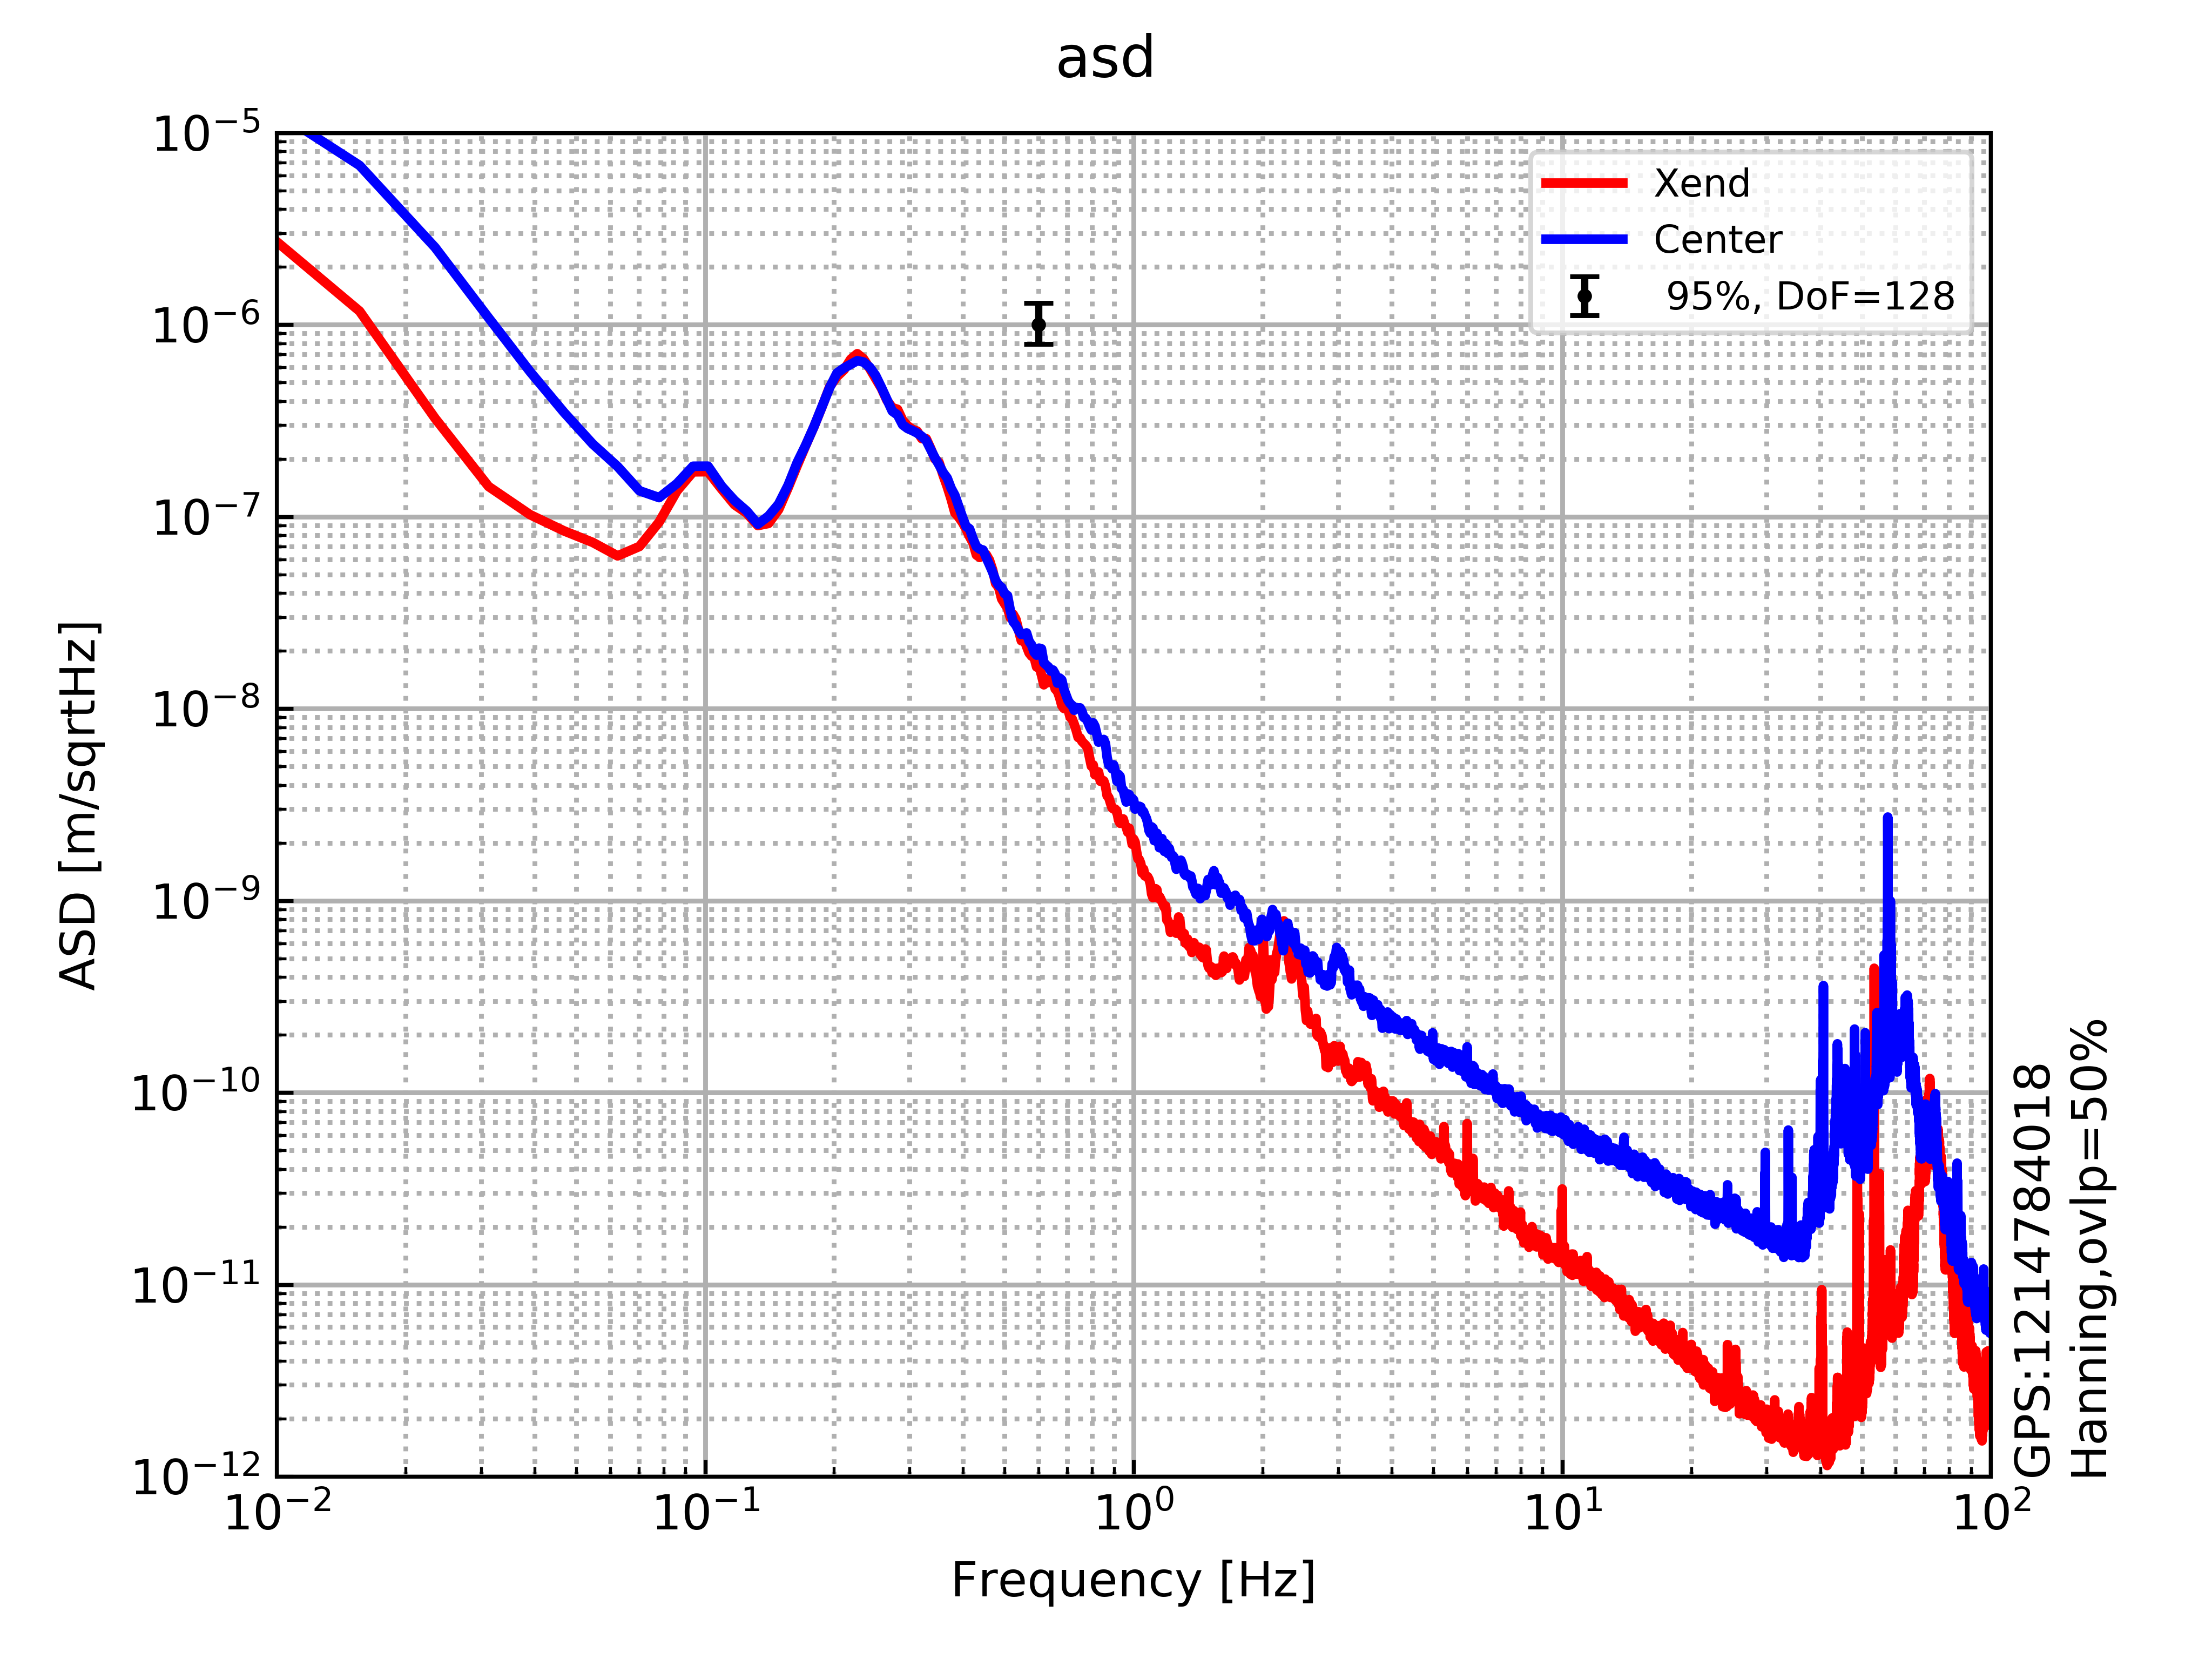
\includegraphics[width=11.5cm]{./XarmDifferentialSpectrum/asd.png}
  \end{center}
  \caption{Xエンドとセンターエリアにおいた地震計のXアーム方向のASD。エラーバーは95%の有意水準。0.1Hz-0.5Hzの帯域では振幅の大きさが同じである。}\label{img:img1}
\end{figure}


\subsubsection{地震計のコヒーレンス}
\begin{figure}[H]
  \begin{center}
    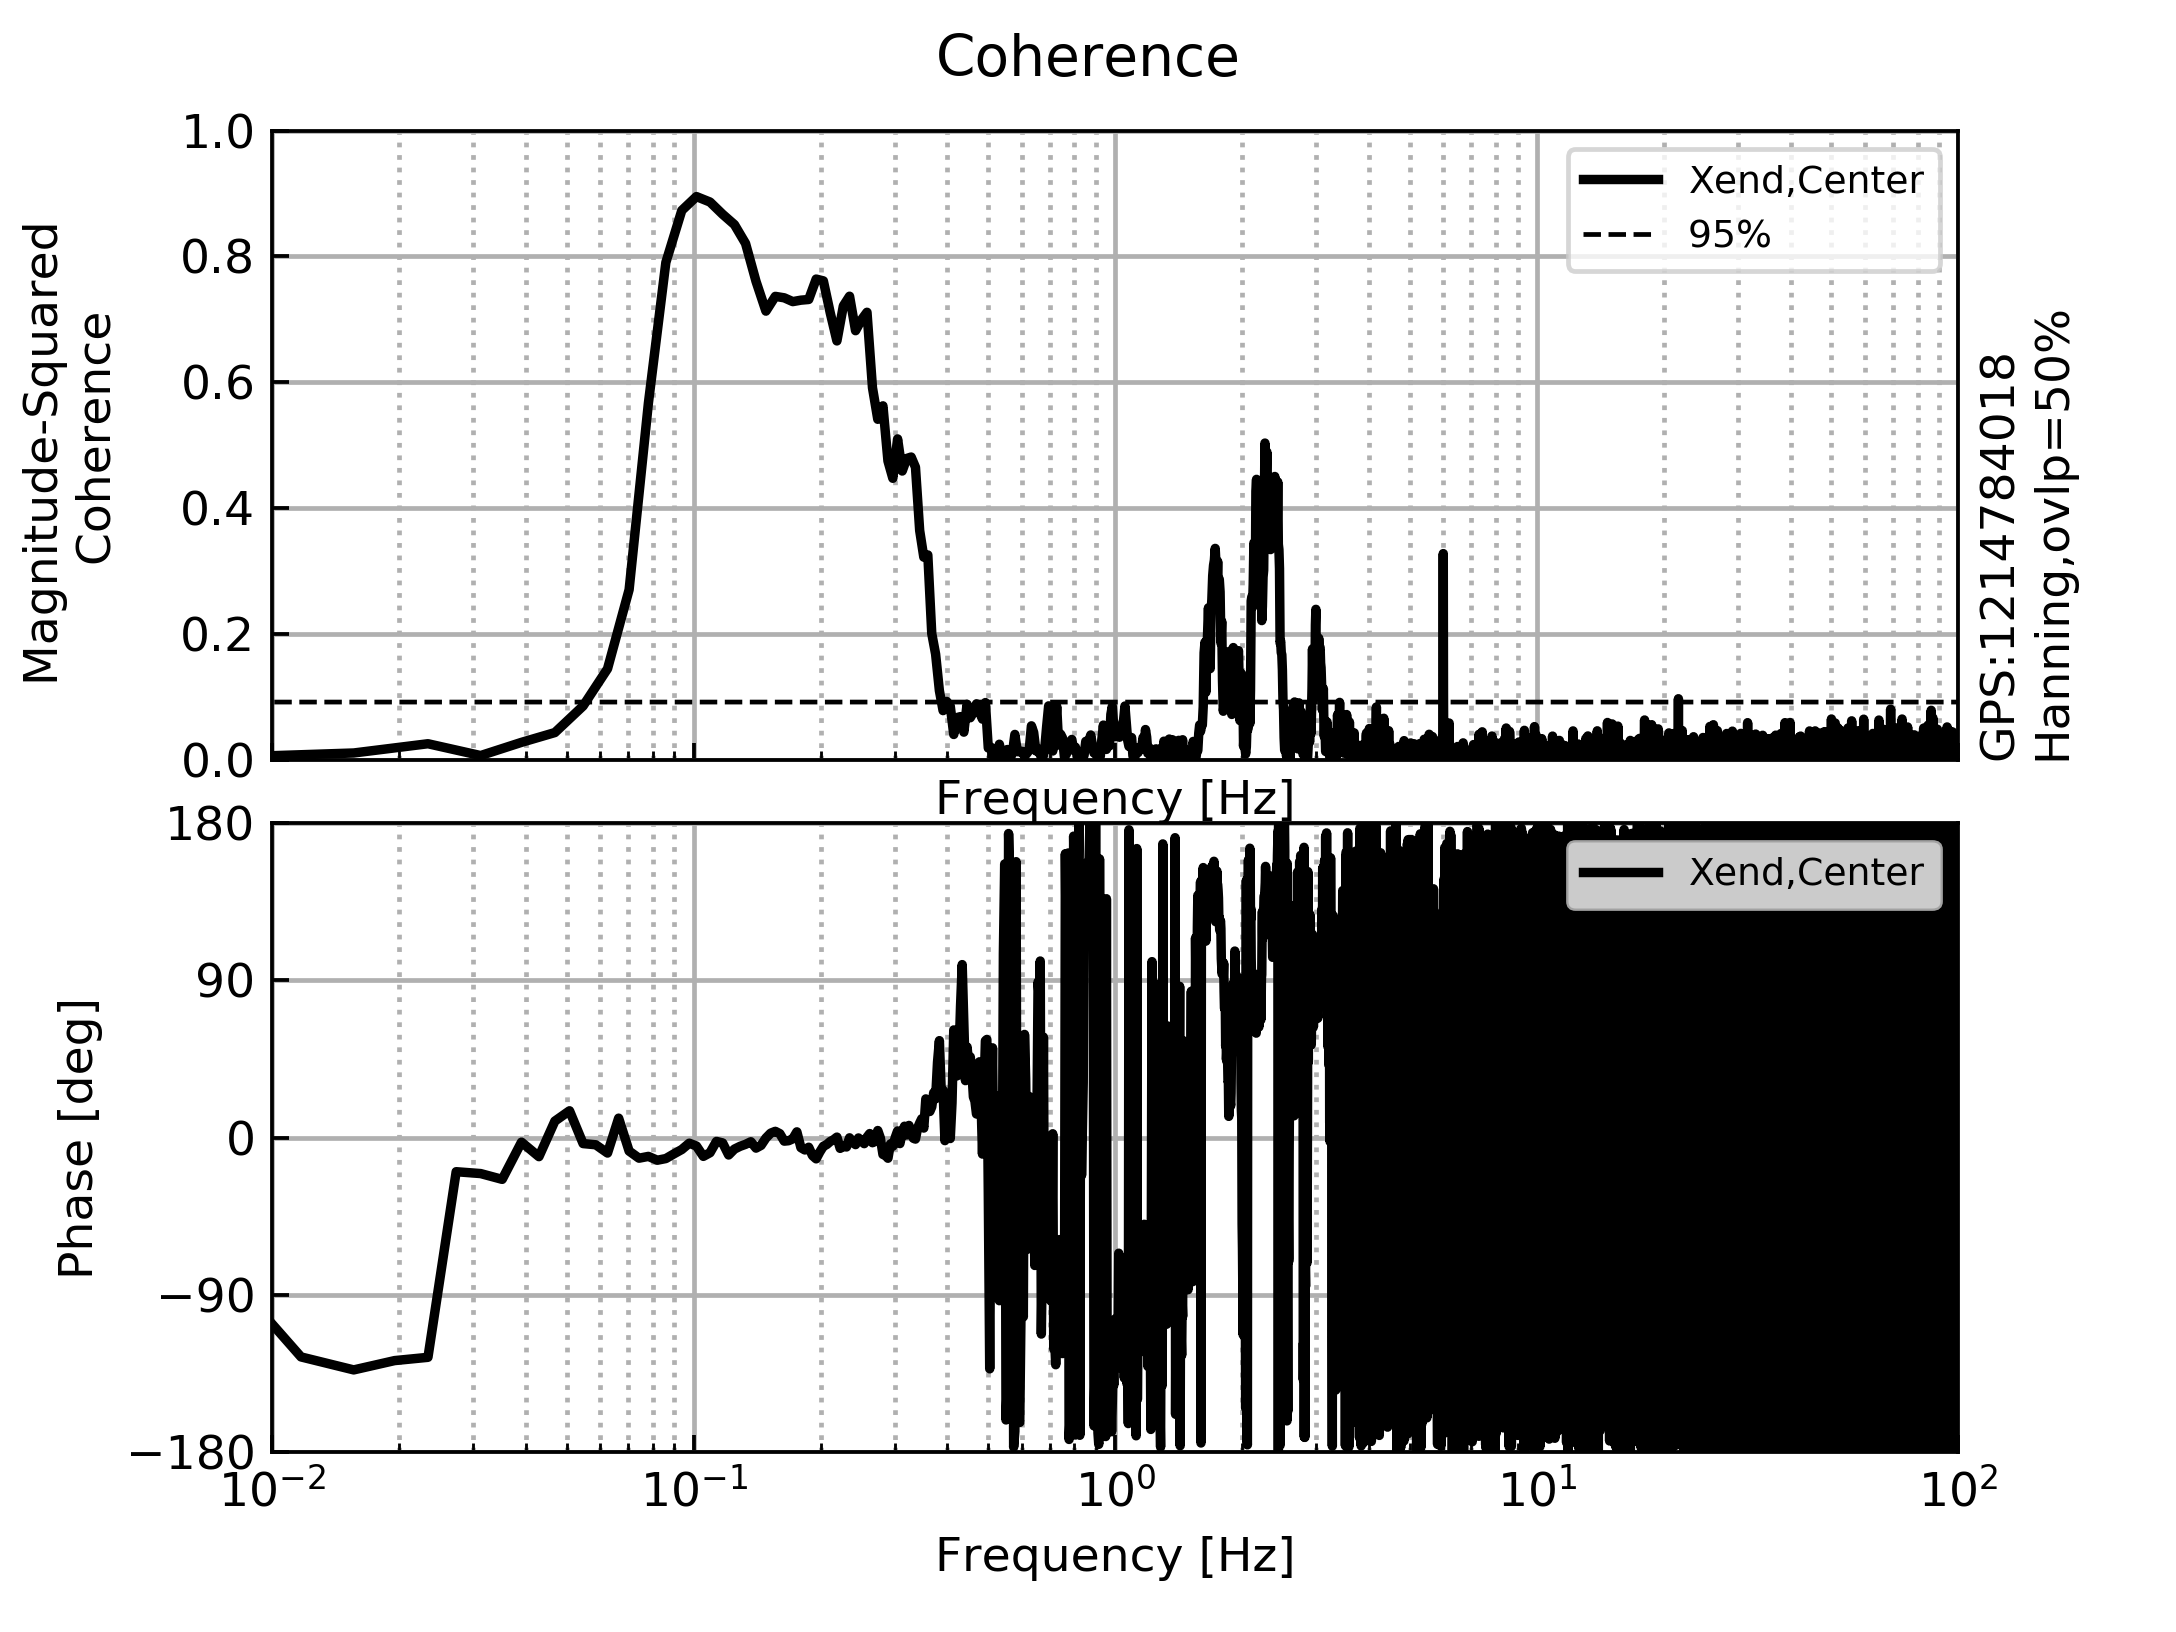
\includegraphics[width=11.5cm]{./XarmDifferentialSpectrum/coh_seismo.png}
  \end{center}
  \caption{Xエンドとセンターエリアにおいた地震計のXアーム方向同士のコヒーレンス。破線は95%の有意水準でコヒーレンスがゼロであるという帰無仮説。すなわちこれ以上では有意にコヒーレンスがあると言える。0.1-0.3Hzと2Hz付近にコヒーレンスがある。前者は脈動,後者は不明。}\label{img:img2}
\end{figure}


図\ref{img:img2}に,Xエンドとセンターの地震計同士のコヒーレンスを示す。コヒーレンスは0.2Hz付近で有意な値をもち、位相が0度であるため,2点が同相で動いていることを意味している。脈動の帯域では,同相成分のほうが逆相成分よりも大きいことを示唆する。

\subsubsection{$\mathrm{CDMR_{seis}}$}
\begin{figure}[H]
  \begin{center}
    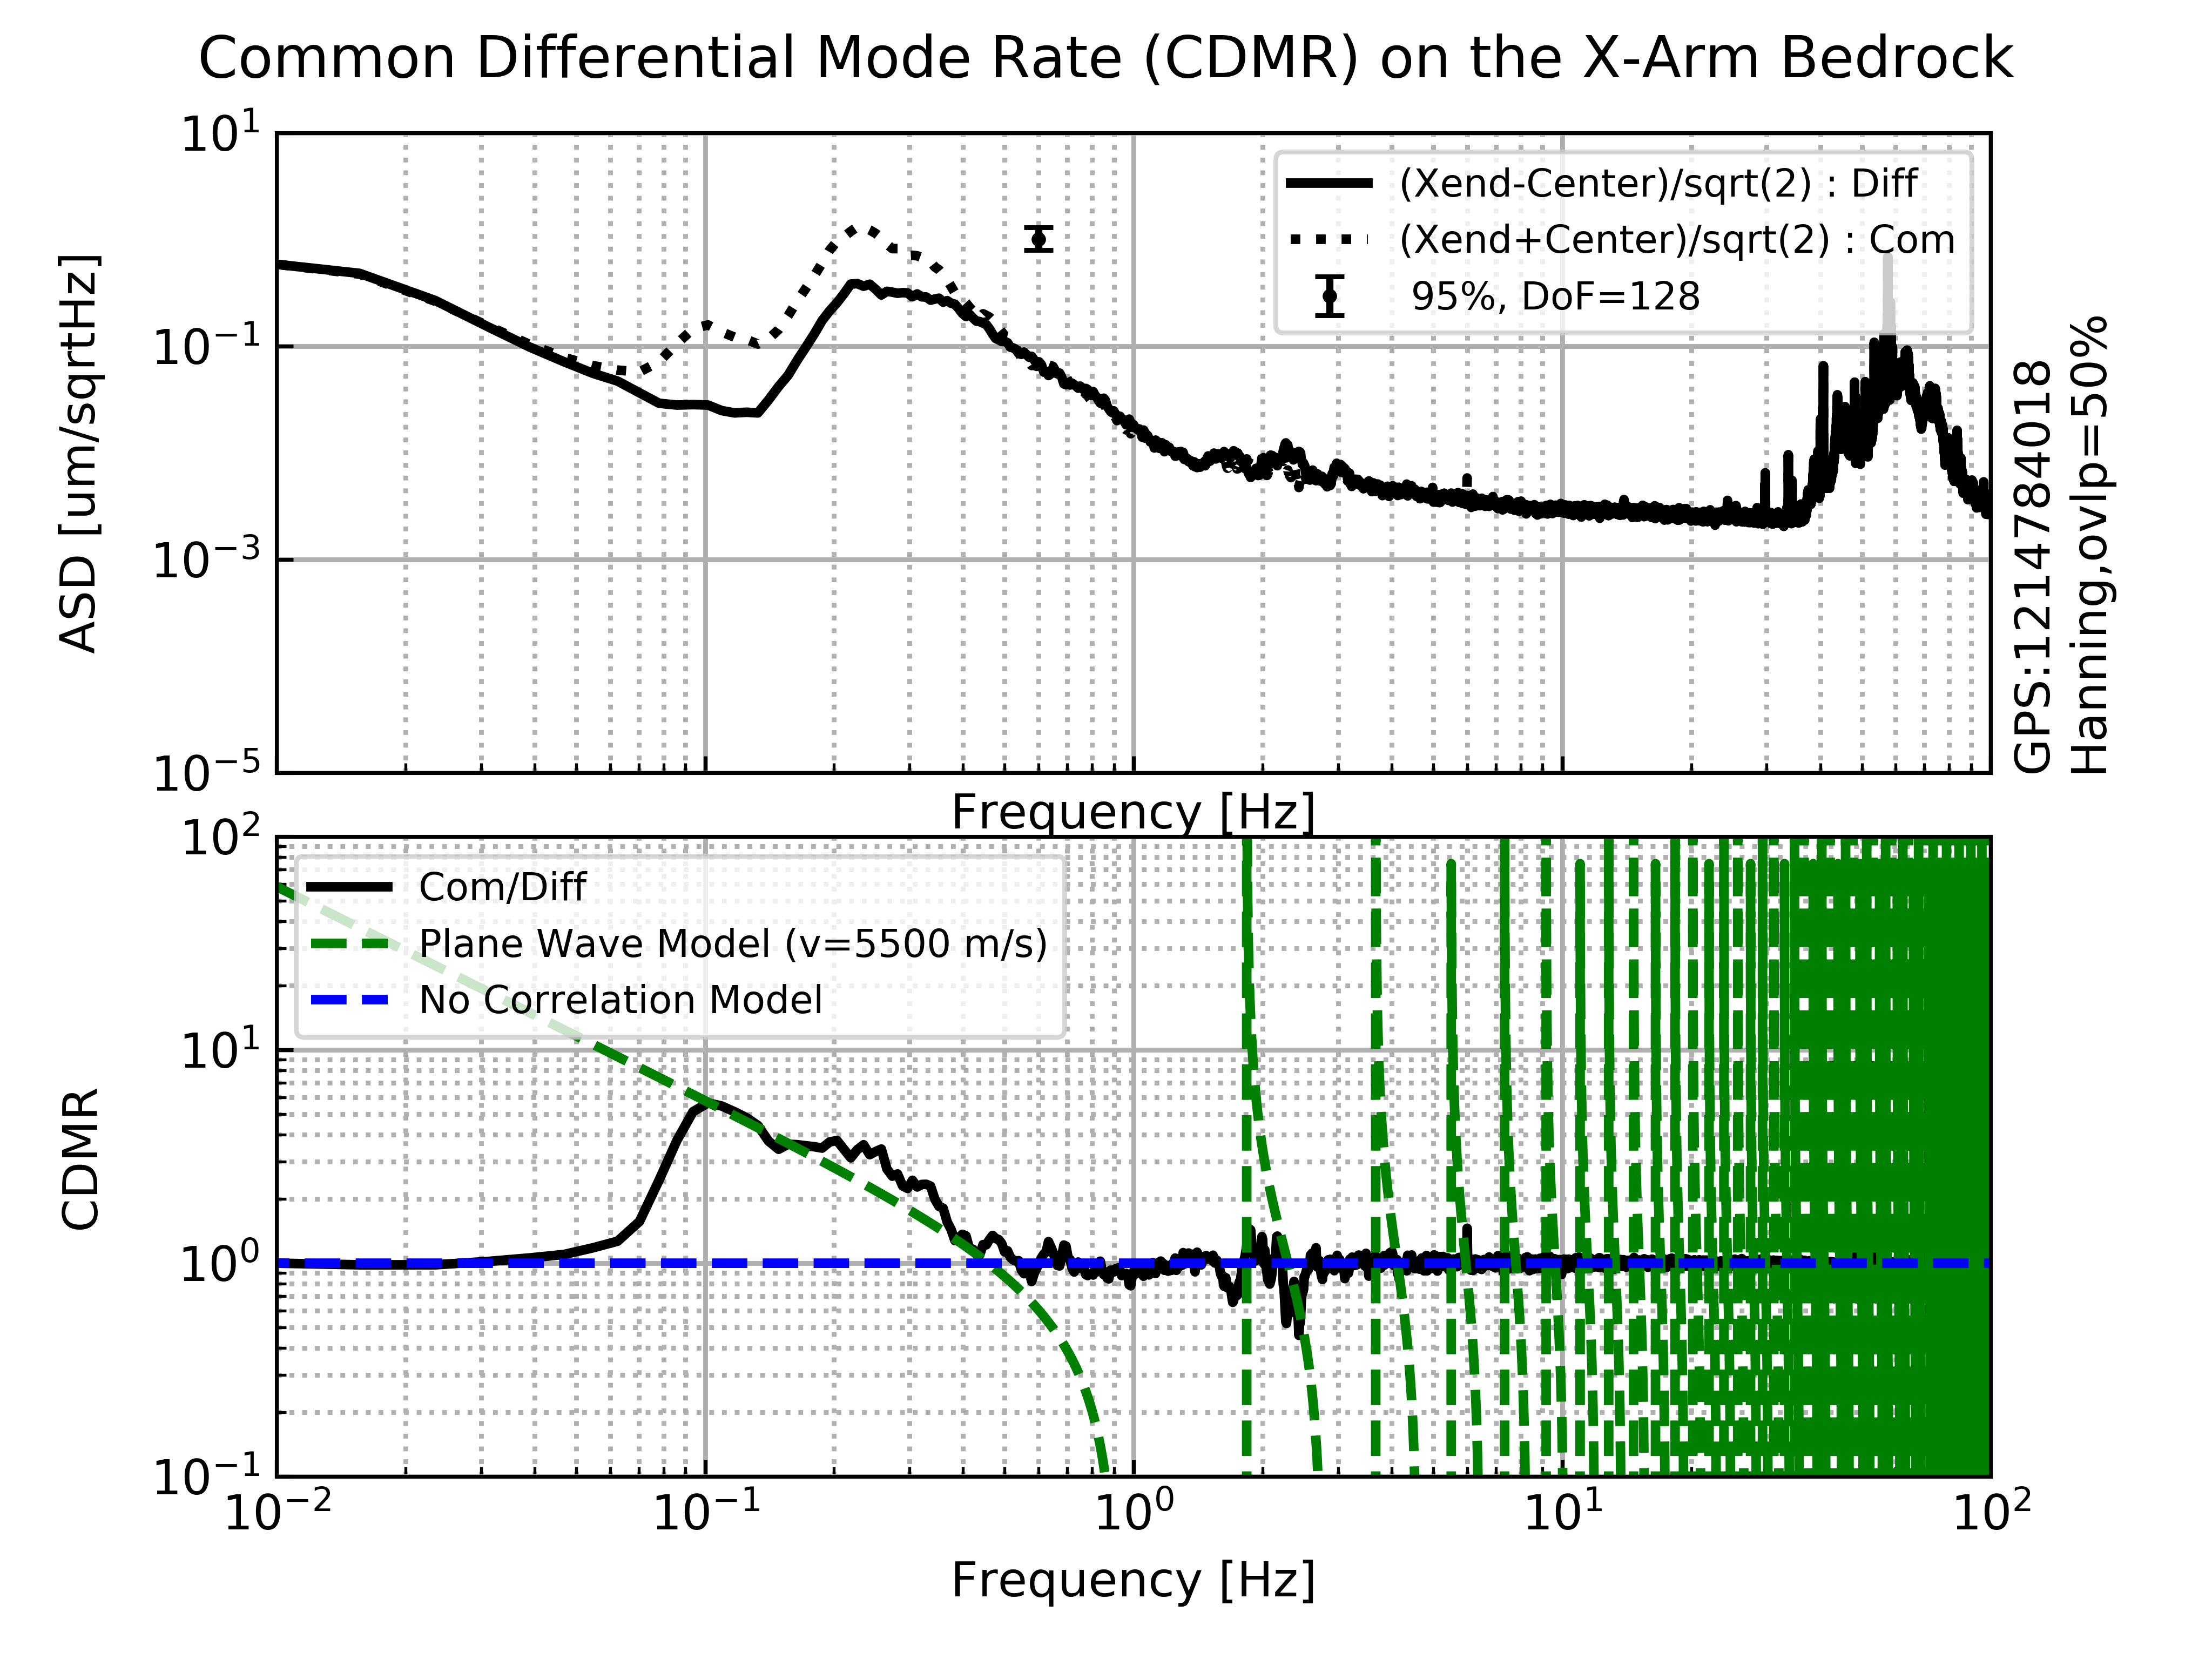
\includegraphics[width=11.5cm]{./XarmDifferentialSpectrum/cmrr_xarm.png}
  \end{center}
  \caption{上図:3km離れた二点の地面振動の同相成分と逆相成分のASD。0.1-0.2Hz付近にピークをもつ脈動では同相成分のほうが逆相成分よりも大きい。下図:同相成分と逆相成分の比(CDMR)。緑色の破線は,位相速度$5500\, \mathrm{m/s}$平面波がXアームを伝搬した場合のCDMRを示す。青色の破線は,相関がない場合のCMDRを示す。脈動はコヒーレンスがあり,波長はKAGRAの基線長よりも長いので,同相雑音が低減されている。}\label{img:img3}
\end{figure}


式\ref{eq:eq18}にP波の位相速度$5500\, \mathrm{m/s}$を代入した\footnote[3]{レイリー波だとおもうけど,とりあえずP波の位相速度で考えておく。}ものを図\ref{img:img3}の下図に緑色の破線で示す。この平面波のモデルと、実測データからもとめたCDMRを比較すると、コヒーレンスがある帯域で一致することがわかる。その他の帯域では,ADCノイズや傾斜ノイズによってコヒーレンスがなくなっているため,式\ref{eq:eq33}より,CDMRは1となる。(図\ref{img:img3}下図の青色破線)。

\subsubsection{$\mathrm{CDMR_{gif}}$}
\begin{figure}[H]
  \begin{center}
    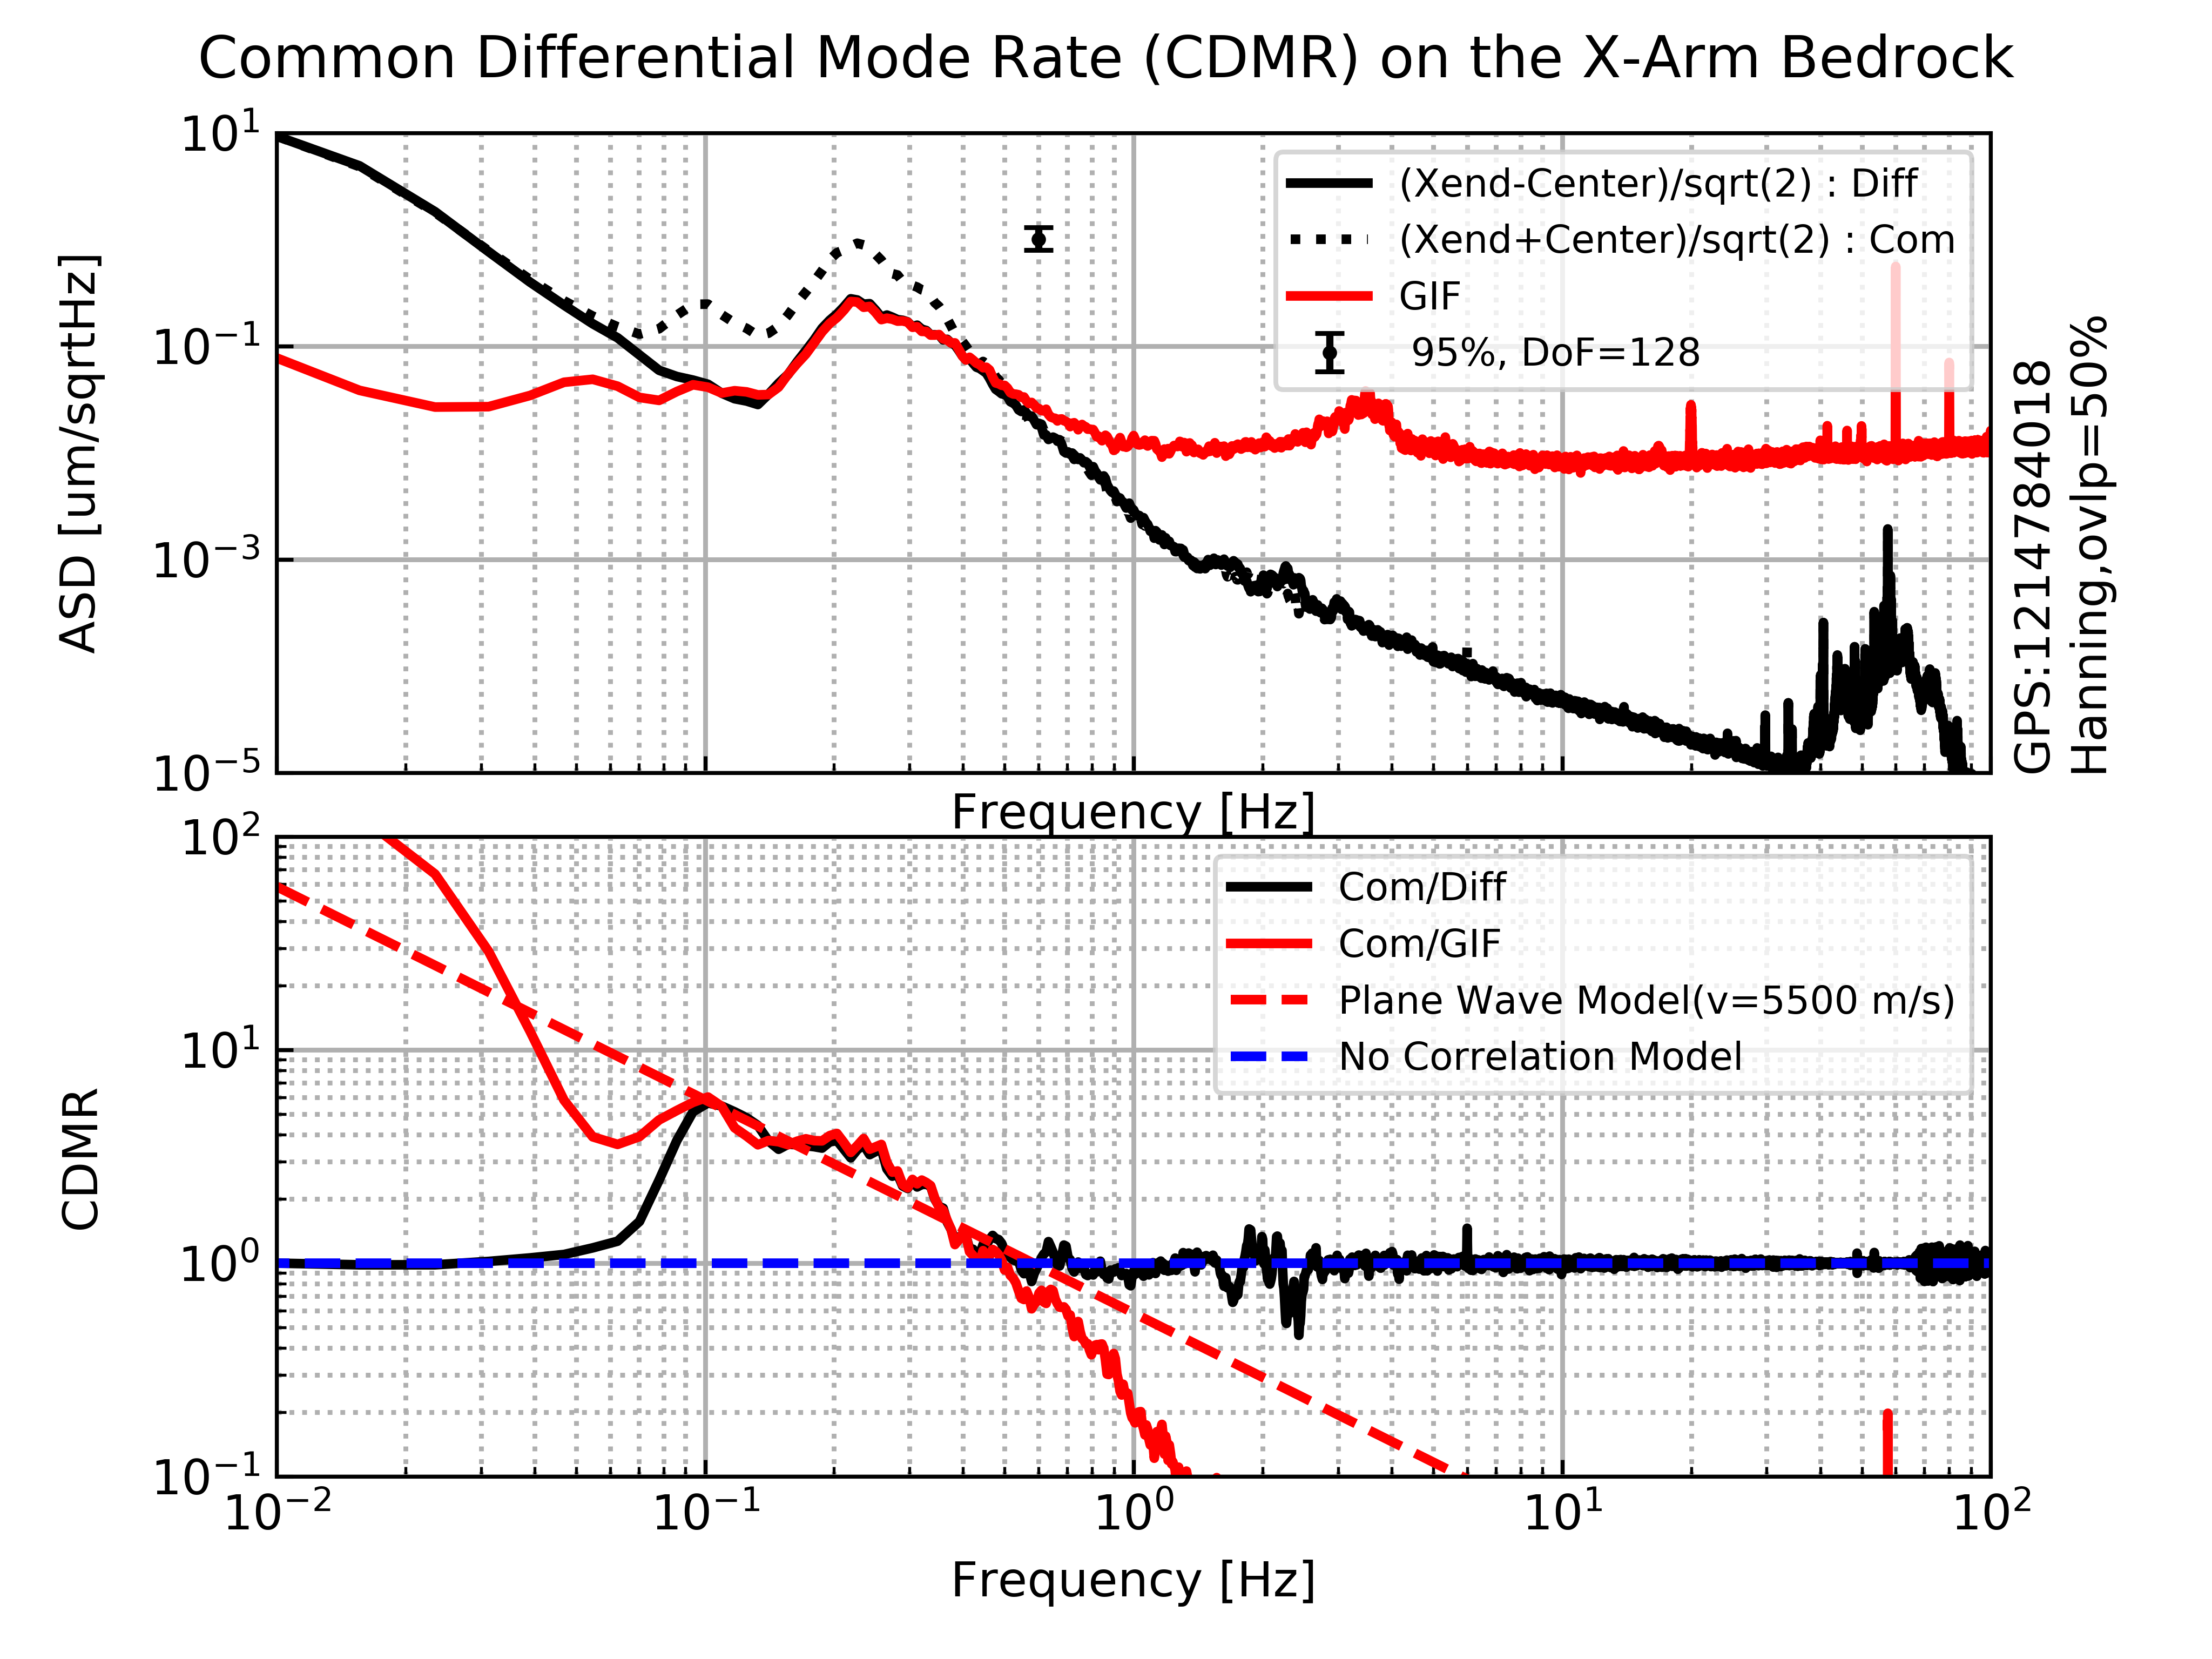
\includegraphics[width=11.5cm]{./XarmDifferentialSpectrum/cmrr_xarm_gif.png}
  \end{center}
  \caption{図\ref{img:img3}にGIFで推定した逆相成分を加えて比較。上図:同相成分と逆相成分の比較。GIFで推定した逆相成分は,脈動の帯域では地震計でもとめたものと一致しているが,低周波では一致しない。これは,図\ref{img:img3}のこの帯域で,CDMRが1で2つの地震計が無相関だったことからも,地震計がローカルなノイズをみていることがわかる。そのためGIFは地震計よりも低周波で感度をもつことが確認できる。下図:逆相成分をGIFで推定したものを加えて比較。式\ref{eq:eq}で表される平面波モデル(赤線の破線)は,図\ref{img:img3}と同様に,脈動の帯域で実測値と一致する。その他の帯域では,先に述べたように,高周波はGIFがADCノイズで,低周波は地震計が傾きノイズをみているため,モデルとは一致しない。
  }\label{img:img4}
\end{figure}

式(\ref{eq:eq39})の位相速度に花崗岩の弾性波速度である5500m/sを代入して図\ref{img:img3}の下図に赤色の破線で示す。地震計と同様に脈動の帯域では平面波のモデルと一致する。それより高周波ではGIFは周波数ノイズに埋もれて地震計の同相成分よりも大きいので,CDMRは平面波のモデルよりも小さくなっている。一方で脈動より低周波では,GIFは基線長伸縮をみているがそれに対応する地震計の逆相成分は,GIFよりも大きい。この帯域では,図\ref{img:img3}で示したように,CDMRが1であったため,地震計同士が無相関で動いている。つまり,傾斜などのローカルなノイズをみていて,基線長伸縮をみていないことがわかる。


\subsection{IMCのCDMR}
IMCのCDMRを求める。図\ref{img:img_imcseis}のように,MCiとMCeにTrilliumCompactを置いた。


\subsubsection{地震計のASD}

\begin{figure}[H]
  \begin{center}
    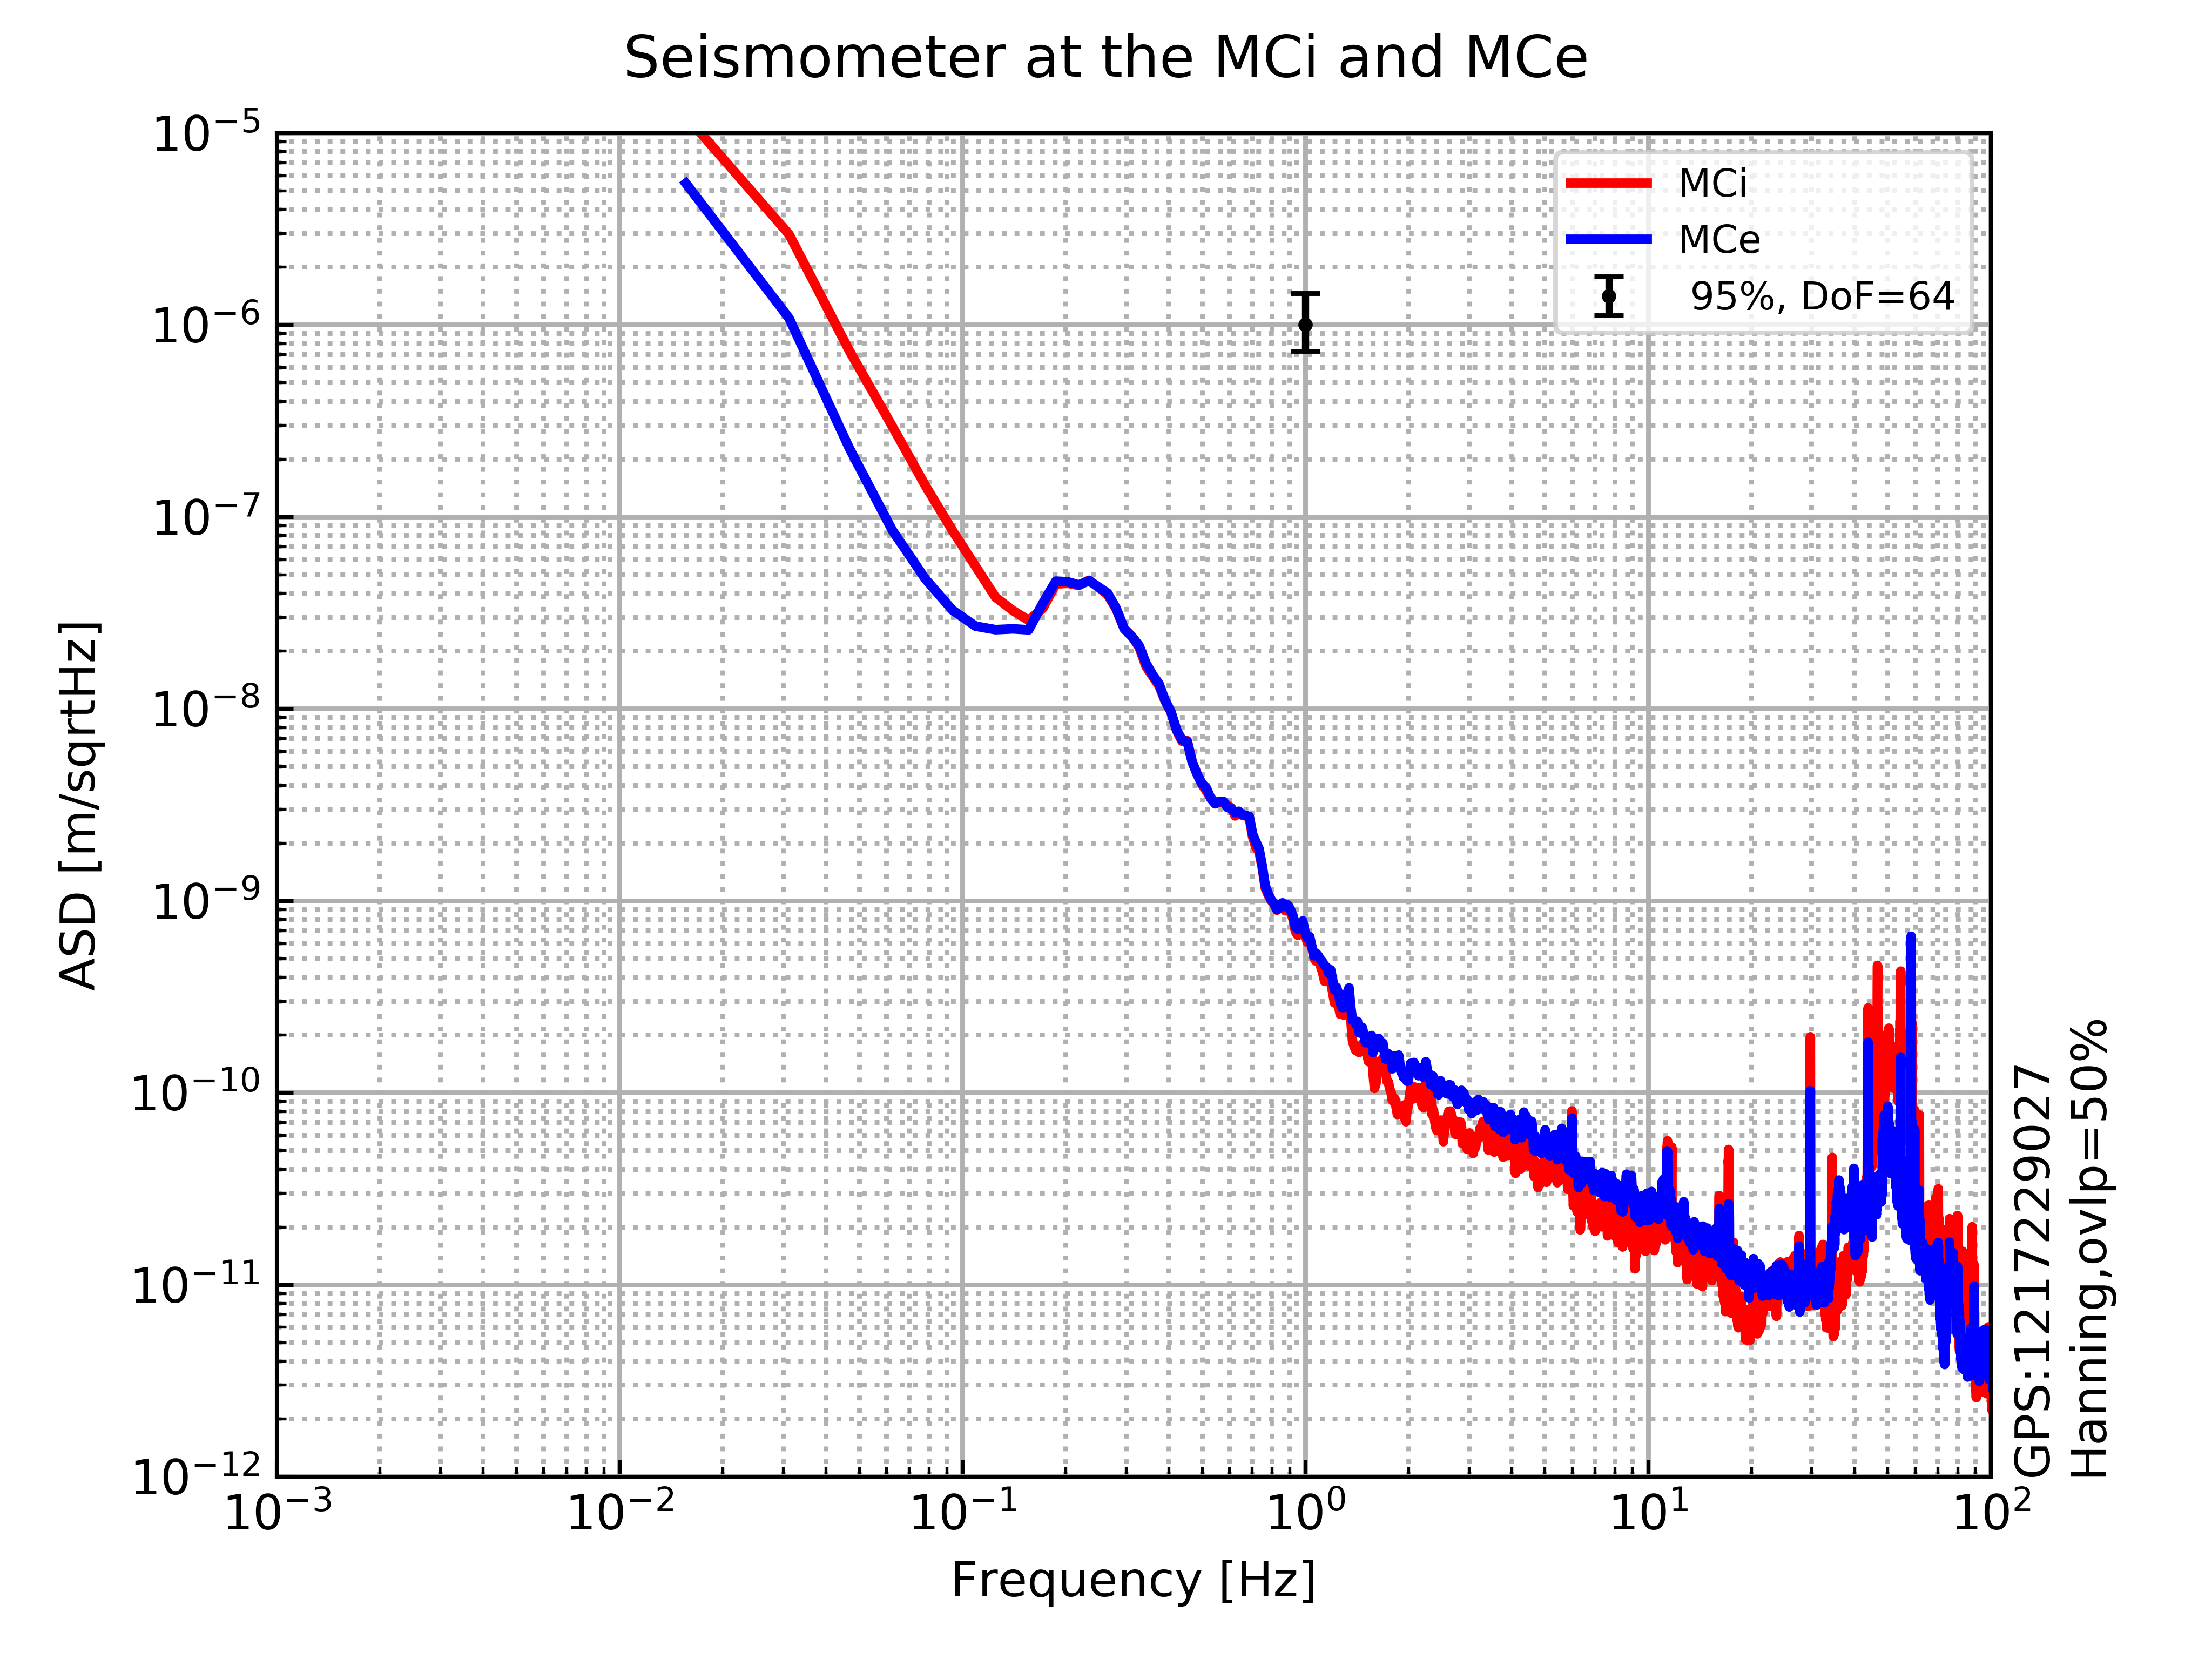
\includegraphics[width=11.5cm]{./XarmDifferentialSpectrum/ASD-MCi_MCe.png}
  \end{center}
  \caption{}\label{img:img_asd_imc}
\end{figure}

\subsubsection{地震計のコヒーレンス}

\begin{figure}[H]
  \begin{center}
    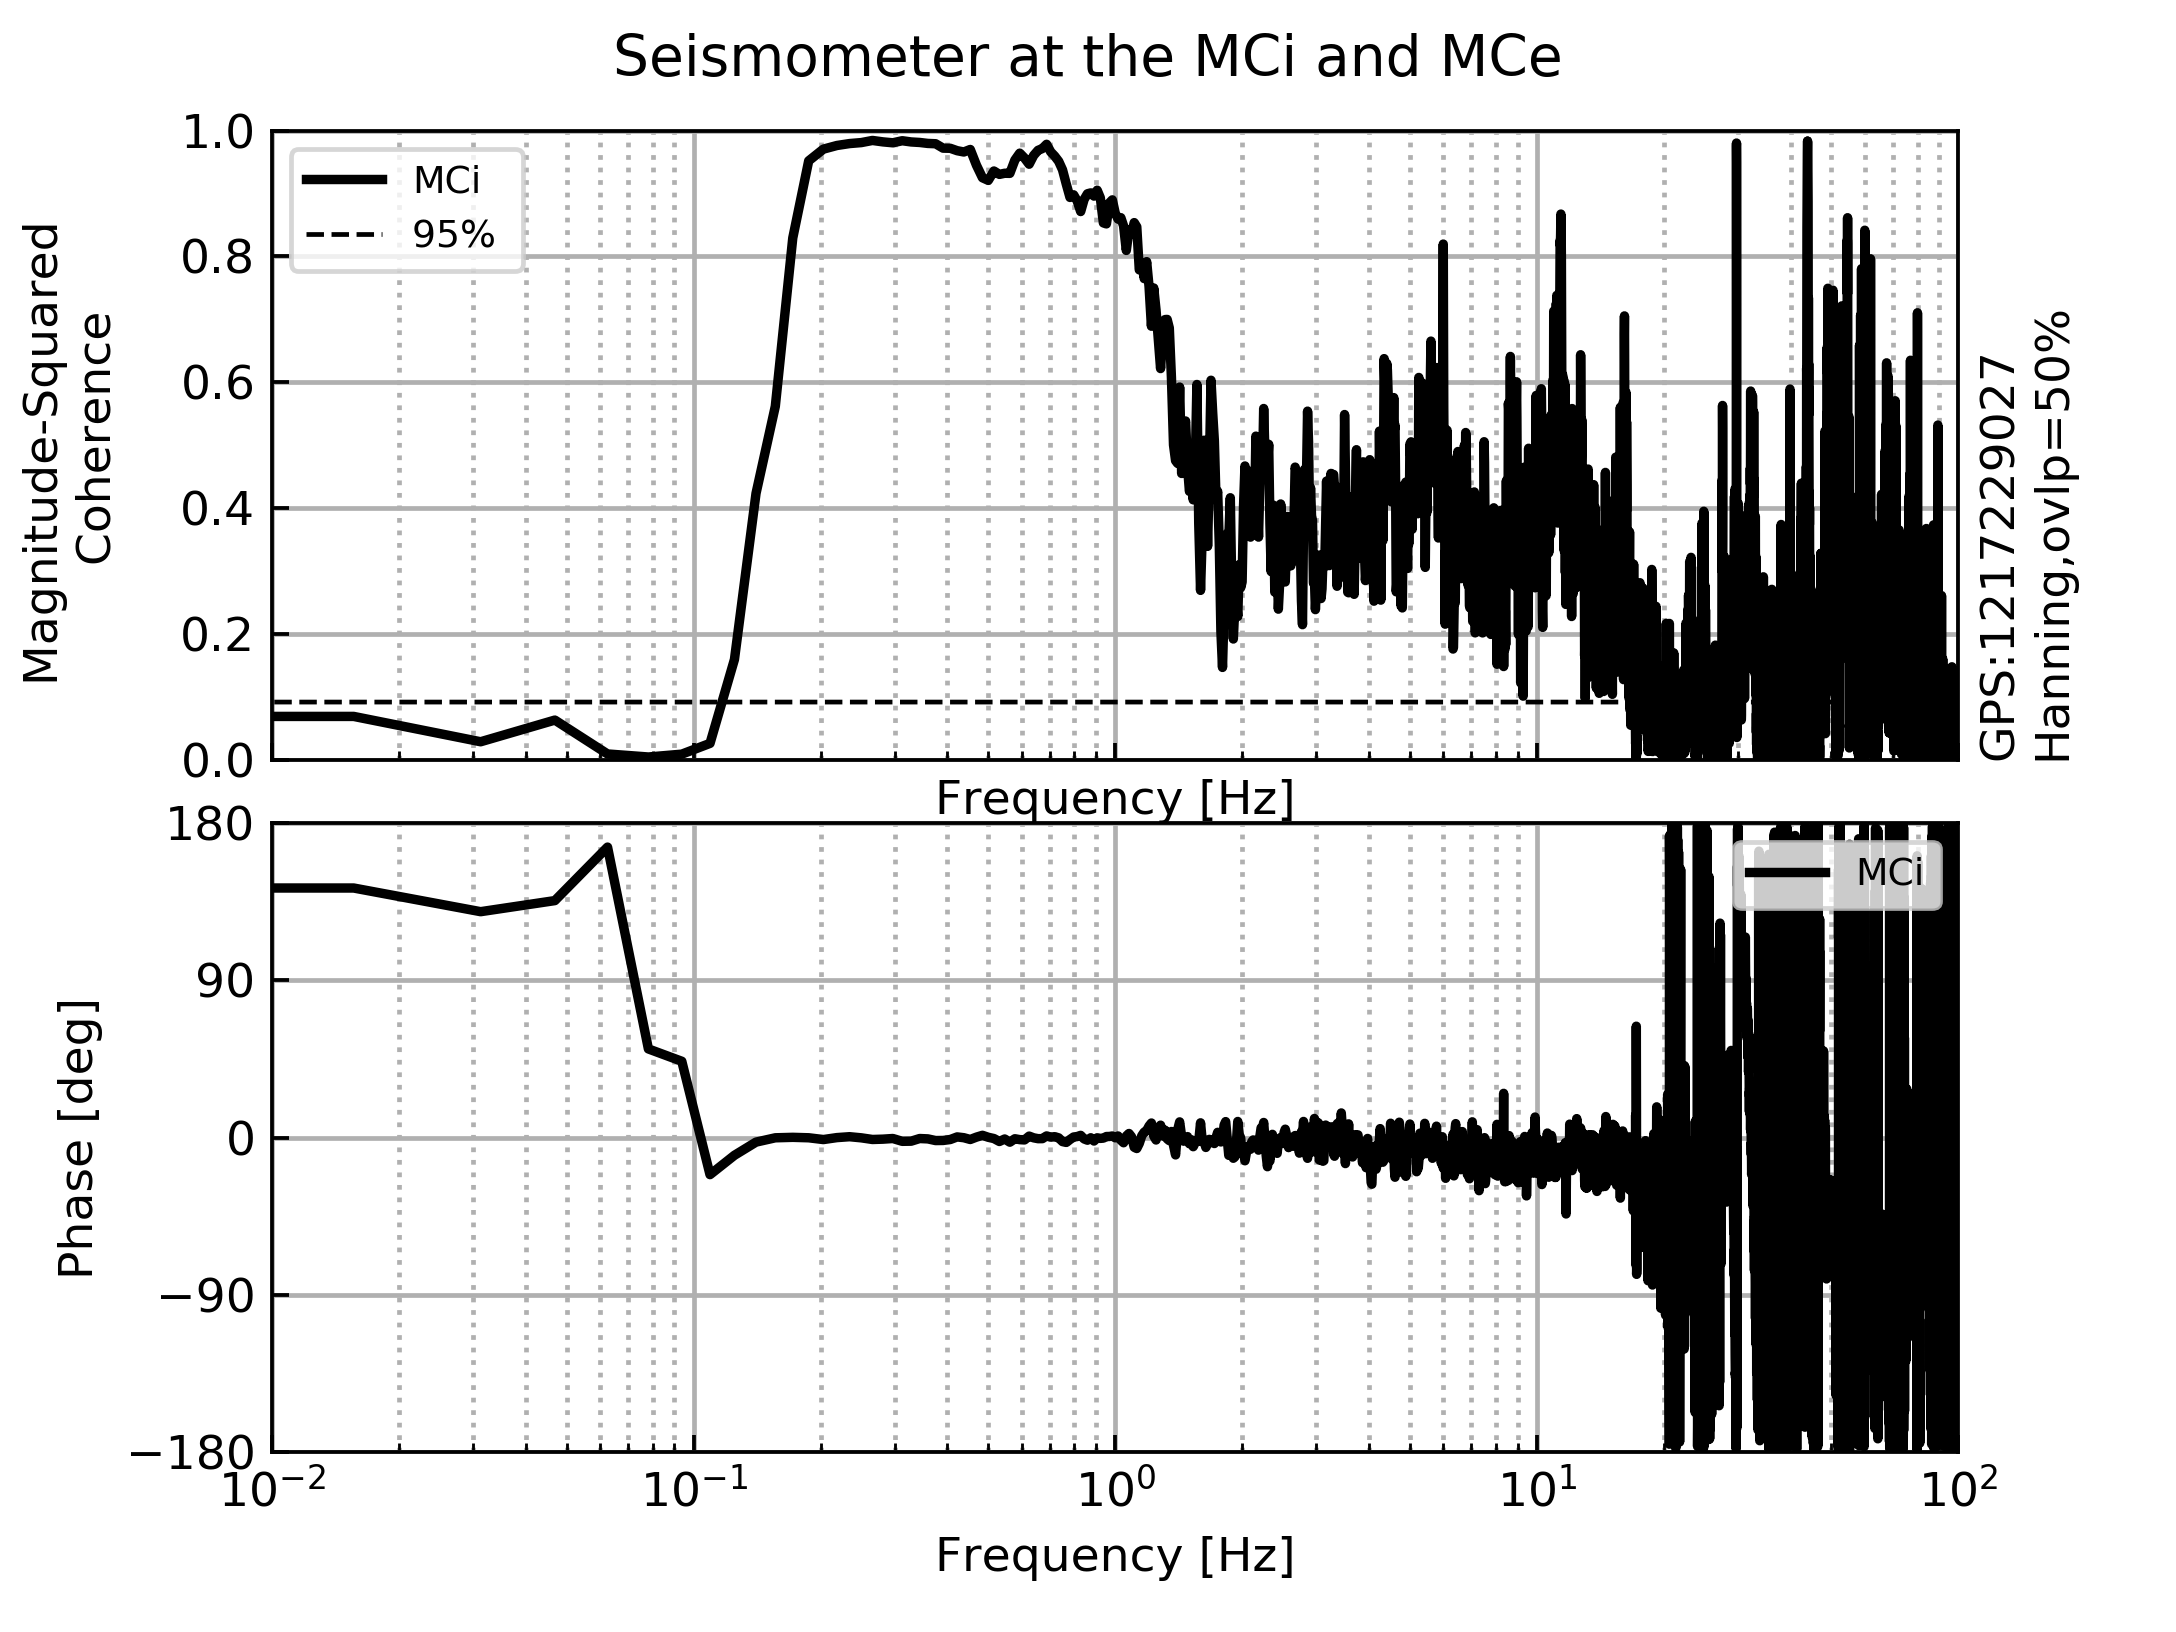
\includegraphics[width=11.5cm]{./XarmDifferentialSpectrum/Coherence-MCi_MCe.png}
  \end{center}
  \caption{}\label{img:img_coherence_imc}
\end{figure}

\subsubsection{$\mathrm{CDMR_{seis}}$}
\begin{figure}[H]
  \begin{center}
    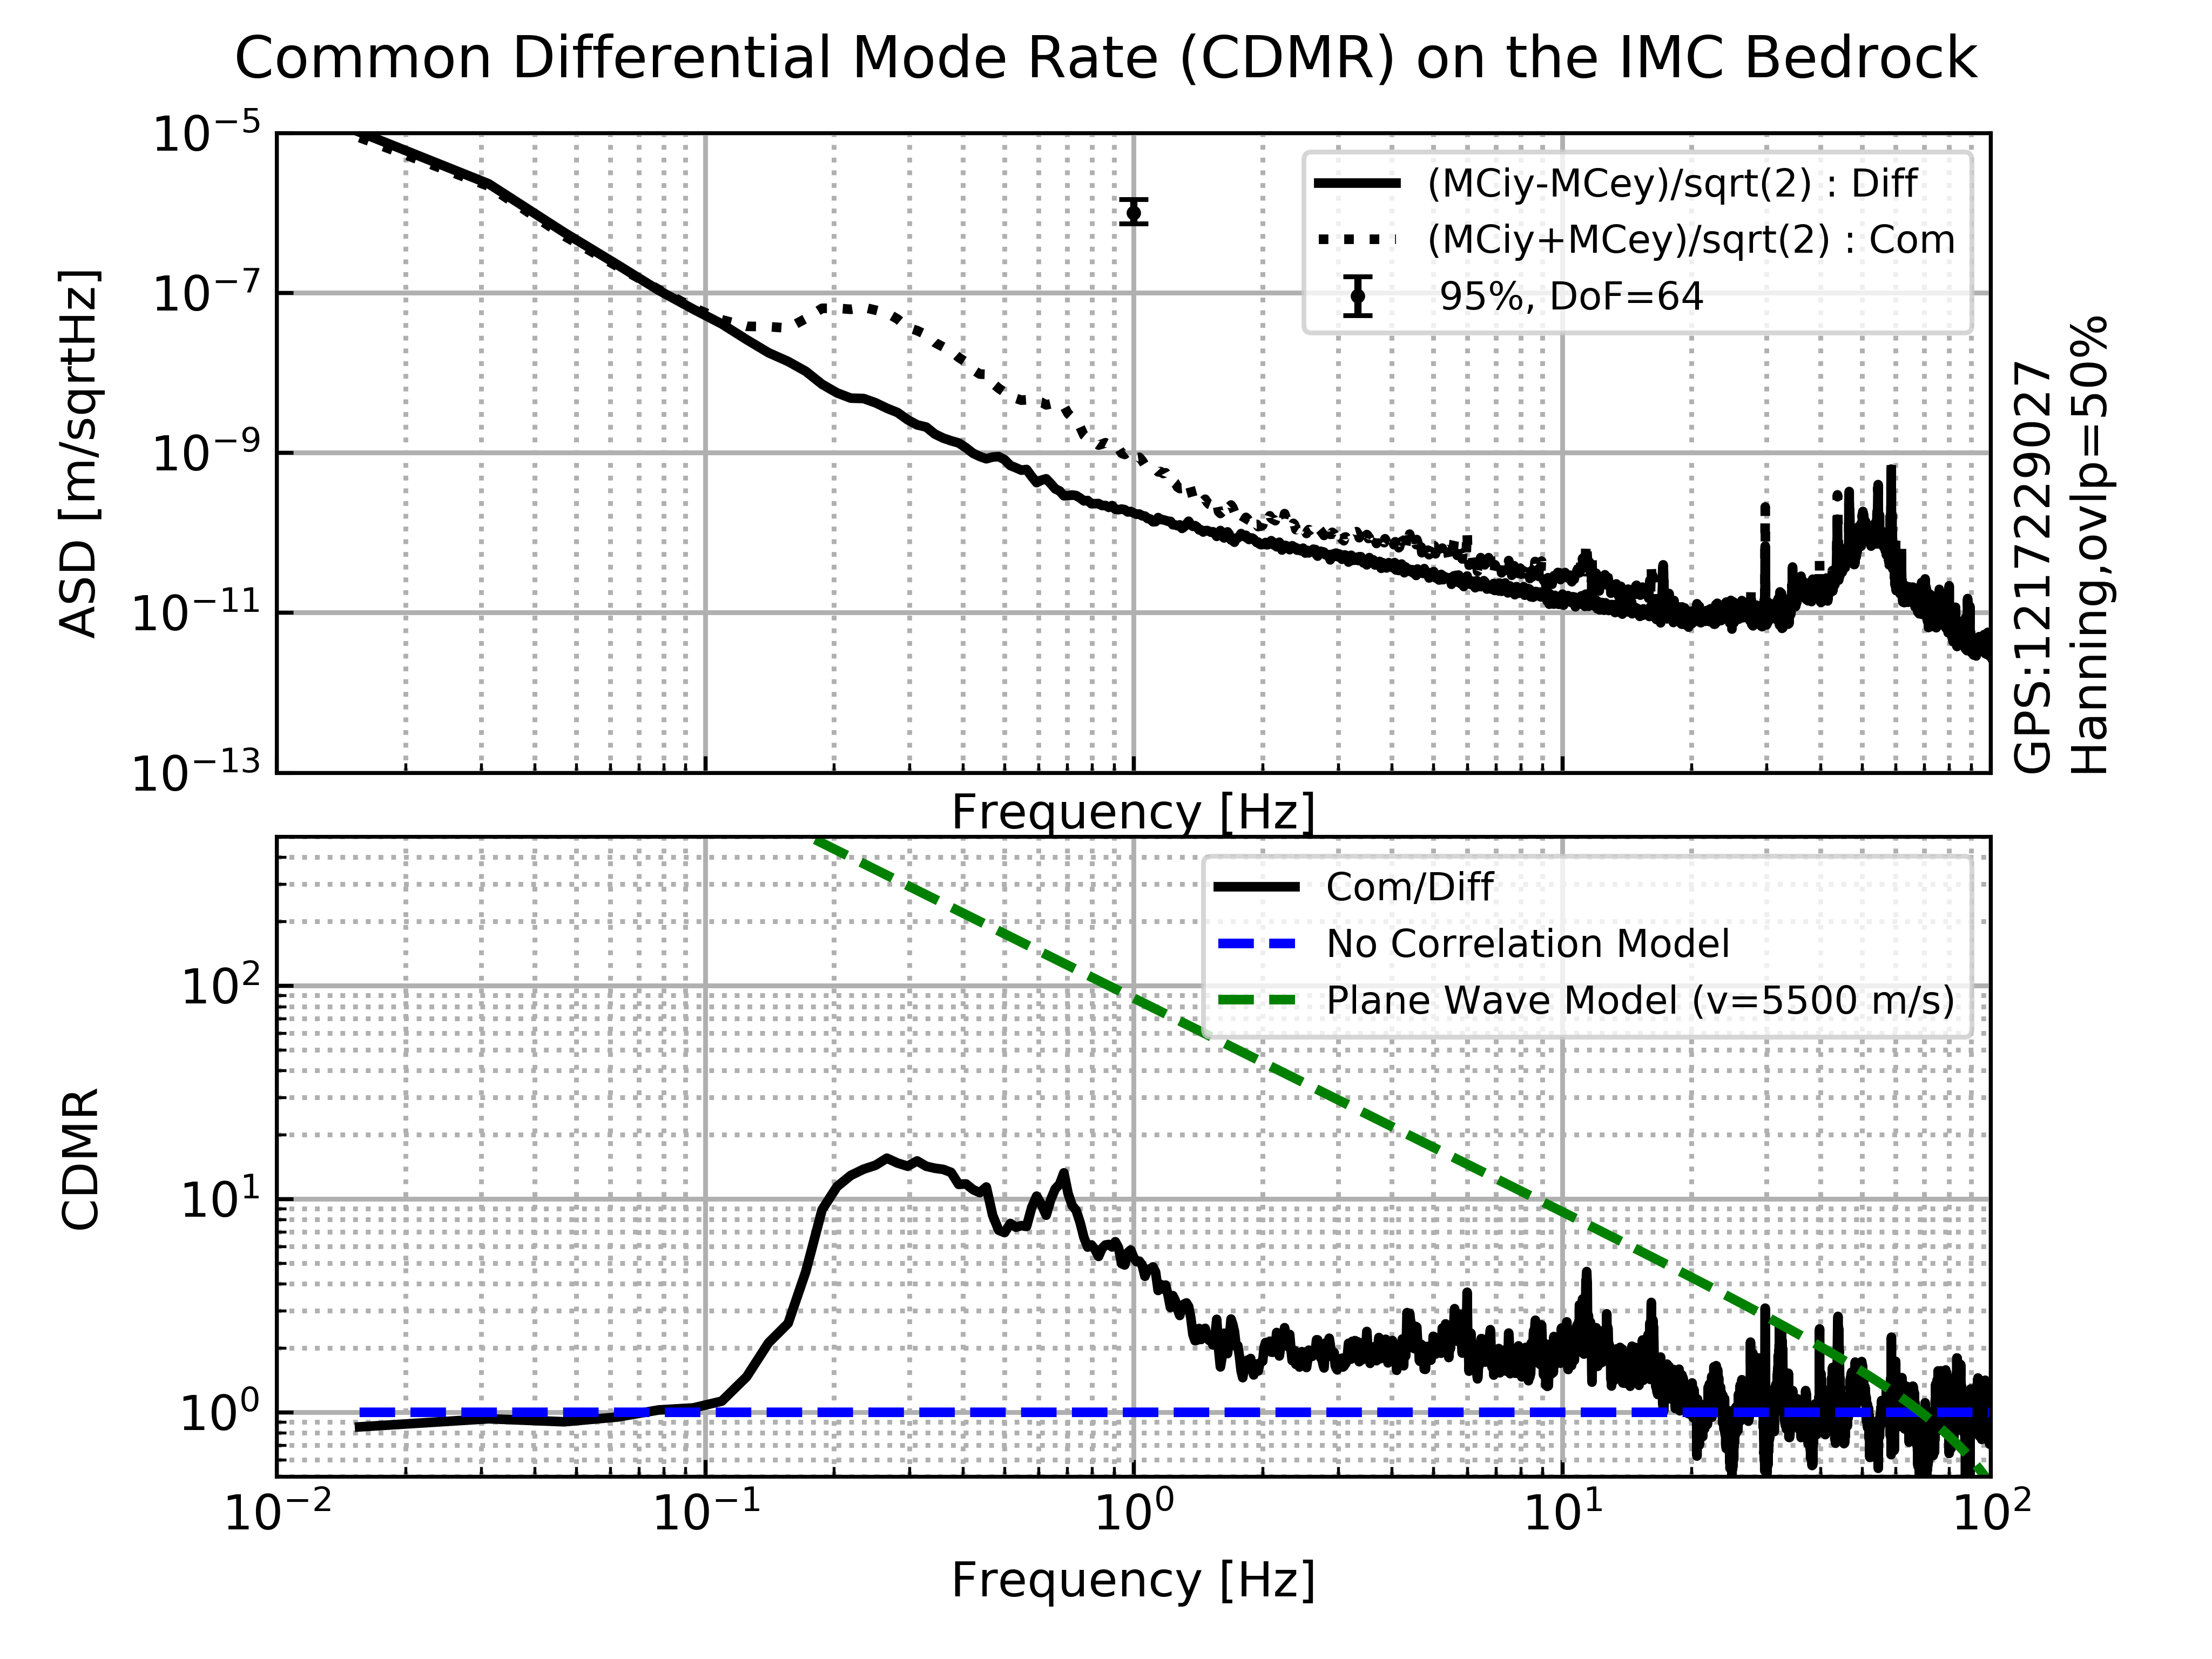
\includegraphics[width=11.5cm]{./XarmDifferentialSpectrum/cdmr_imc.png}
  \end{center}
  \caption{}\label{img:img_cdmr_imc}
\end{figure}




\subsection{長期データ}
長期間の基線長伸縮スペクトルをここでのべる。今後KAGRAの基線長伸縮として引用できるようなもの。一年をとおしてデータを解析してみる。平均的なスペクトルを知りたいので地震や台風のときは除く、もしくは「うるさいとき」という感じで、スペクトルを乗せる。


\subsection{環境変動によるXアームの基線長伸縮}
波浪や地震、気圧・水圧などの環境変化によって基線長伸縮がどう影響をうけるか述べる。

\subsubsection{波浪}

\subsubsection{地震}

\subsubsection{気圧}

\subsubsection{水圧}

\subsection{まとめ}
本章では、同相成分と逆相成分の比であるCommon Differential Mode Ratio (CDMR)という量を定義して、Xアームを平面波が通過している簡単なモデルと、実測データを比較した。その結果、脈動ではセンターとXエンド同士で有意なコヒーレンスがあった。この帯域では、平面波のモデルと実測データが一致し、2点は同相で動いていることがわかった。そして、CDMRを計算すると、最大で逆相成分が同相成分の1/4になっており、3kmの基線長でも逆相成分の低減が確認できた。


また、地震計とひずみ計の比較もおこなった。

ひずみ計は1500mの基線長伸縮を直接みており、地震計とは異なって、原理的には地面の傾斜成分は並進方向にカップルしないため、低周波


